\documentclass[12pt]{scrartcl}
\usepackage[pretty,polish]{mystd}
\title{Rozwiązania równania potencjału grawitacyjnego z użyciem FEM}
\author{Michał Dobranowski}
\date{22 grudnia 2023}

\begin{document}
    \maketitle

    \section*{Sformułowanie silne}
    Dane jest następujące równanie
    \begin{equation} \label{eq:main}
        \frac{\d{}^2 \Phi(x)}{\d x^2} = 4\pi G\rho(x),
    \end{equation}
    gdzie
    \[ \rho(x) = \begin{cases}
        0, & \text{dla } x \in [0, 1] \\
        1, & \text{dla } x \in (1, 2] \\
        0, & \text{dla } x \in (2, 3]
    \end{cases}, \]
    przy warunkach brzegowych
    \[ \Phi(0) = 5, \quad \Phi(3) = 4. \]
    Szukana jest funkcja $\Phi : [0, 3] \to \RR$.

    \section*{Sformułowanie słabe (wariacyjne)}
    Mnożąc równanie \ref{eq:main} obustronnie przez funkcję testową $v$ i całkując na dziedzinie $[0, 3]$ otrzymujemy
    \[ \int_0^3 \Phi'' v \d x = 4\pi G \int_0^3 \rho v \d x, \]
    co, korzystając z definicji $\rho$, możemy zapisać jako
    \[ \int_0^3 \Phi'' v \d x = 4\pi G \int_1^2 v \d x. \]
    Teraz całkujemy przez części
    \[ \big[\Phi' v\big]_0^3 - \int_0^3 \Phi' v' \d x = 4\pi G \int_1^2 v \d x. \]
    Ponieważ obustronnie zadano warunek Dirichleta, funkcja testowa $v$ zeruje się na brzegu dziedziny, więc
    \[ -\int_0^3 \Phi' v' \d x = 4\pi G \int_1^2 v \d x. \]

    \newcommand{\tPhi}{\widetilde{\Phi}}
    Chcemy szukać rozwiązań w formie $\Phi = w + \tPhi$, gdzie $w(0) = w(3) = 0$. Łatwo zauważyć, że taką funkcją jest $\tPhi(x) = 5 - \frac{x}{3}$. Podstawiamy i oznaczamy:
    \[ -\int_0^3 (w' + \tPhi') v' \d x = 4\pi G \int_1^2 v \d x, \]
    \begin{equation}
        \underbrace{-\int_0^3 w'v' \d x}_{\let\scriptstyle\textstyle \substack{B(w, v)}} = \underbrace{4\pi G \int_1^2 v \d x + \int_0^3 \tPhi'v' \d x}_{\let\scriptstyle\textstyle \substack{L(v)}}.
    \end{equation}

    \section*{Dyskretyzacja problemu}
    Dzielimy dziedzinę $[0, 3]$ na $n$ przedziałów $(x_j, x_{j+1})$ o długości $h = \frac{3}{n}$ takich, że
    \[ x_j = 3 \cdot \frac{j}{n}, \quad\text{dla } j \in \{0, \ldots, n\}. \]
    Będziemy używać funkcji bazowych $e_i$ zdefiniowanych następująco
    \[ e_i = \begin{cases}
        \frac{x - x_{i-1}}{h}, &\text{dla } x \in (x_{i-1}, x_i), \\
        \frac{x_{i+1} - x}{h}, &\text{dla } x \in (x_i, x_{i+1}), \\
        0, & \text{w innym przypadku.}
    \end{cases} \]
    Pochodna takiej funkcji to
    \[ e_i' = \begin{cases}
        \frac{1}{h}, &\text{dla } x \in (x_{i-1}, x_i), \\
        -\frac{1}{h}, &\text{dla } x \in (x_i, x_{i+1}), \\
        0, & \text{w innym przypadku.}
    \end{cases} \]

    Funkcja $w$ będzie przybliżana przez pewną kombinację liniową funkcji bazowych $e_i$. Ograniczymy również nieskończenie wymiarową przestrzeń funkcji testujących $V$ do skończenie wymiarowej przestrzeni funkcji bazowych $V_h \subset V$. Niech zbiór funkcji $v_i = e_i$ będzie bazą tej przestrzeni. Dla każdego $j \in \{0, \ldots, n\}$ mamy więc
    \[ B\left(\sum_{i=0}^n \alpha_i e_i, v_j\right) = L(v_j). \]
    Ze względu na dwuliniowość $B$, możemy przekształcić powyższy układ równań do postaci
    \[ \sum_{i=0}^n \alpha_i B\left(e_i, v_j\right) = L(v_j), \quad j \in \{1, \ldots, n\}, \]
    czyli, wykorzystując $v_i = e_i$,
    \[ \begin{bNiceMatrix}
        B(e_0, e_0) & B(e_1, e_0) & \Cdots & B(e_n, e_0) \\
        B(e_0, e_1) & B(e_1, e_1) & \Cdots & B(e_n, e_1) \\
        \Vdots & \Vdots & \Ddots & \Vdots \\
        B(e_0, e_n) & B(e_1, e_n) & \Cdots & B(e_n, e_n)
    \end{bNiceMatrix} \begin{bNiceMatrix}
        \alpha_0 \\
        \alpha_1 \\
        \Vdots \\
        \alpha_n
    \end{bNiceMatrix} = \begin{bNiceMatrix}
        L(e_0) \\
        L(e_1) \\
        \Vdots \\
        L(e_n)
    \end{bNiceMatrix}. \]

    Ze względu na warunki Dirichleta, musimy zapewnić, że $\alpha_0 = \alpha_n = 0$. Usuwamy odpowiednie wiersze i kolumny macierzy otrzymując
    \[ \begin{bNiceMatrix}
        B(e_1, e_1) & B(e_2, e_1) & \Cdots & B(e_{n-1}, e_1) \\
        B(e_1, e_2) & B(e_2, e_2) & \Cdots & B(e_{n-1}, e_2) \\
        \Vdots & \Vdots & \Ddots & \Vdots \\
        B(e_1, e_{n-1}) & B(e_2, e_{n-1}) & \Cdots & B(e_{n-1}, e_{n-1})
    \end{bNiceMatrix} \begin{bNiceMatrix}
        \alpha_1 \\
        \alpha_2 \\
        \Vdots \\
        \alpha_{n-1}
    \end{bNiceMatrix} = \begin{bNiceMatrix}
        L(e_1) \\
        L(e_2) \\
        \Vdots \\
        L(e_{n-1})
    \end{bNiceMatrix}. \]

    \subsection*{Uproszczenie układu równań}
    Można zauważyć, że ze względu na konstrukcję funkcji $e_i$, $B(e_i, e_j) = 0$ dla każdej pary $i, j$, dla której $|i - j| \geq 2$. Dodatkowo, $B(e_i, e_j) = B(e_j, e_i)$.

    \section*{Wynik}
    Dla $G = 1$ (dla prawdziwej stałej grawitacyjnej wykres jest bliski prostej) otrzymano poniższej narysowaną funkcję.

    \begin{figure}[H]
        \centering
        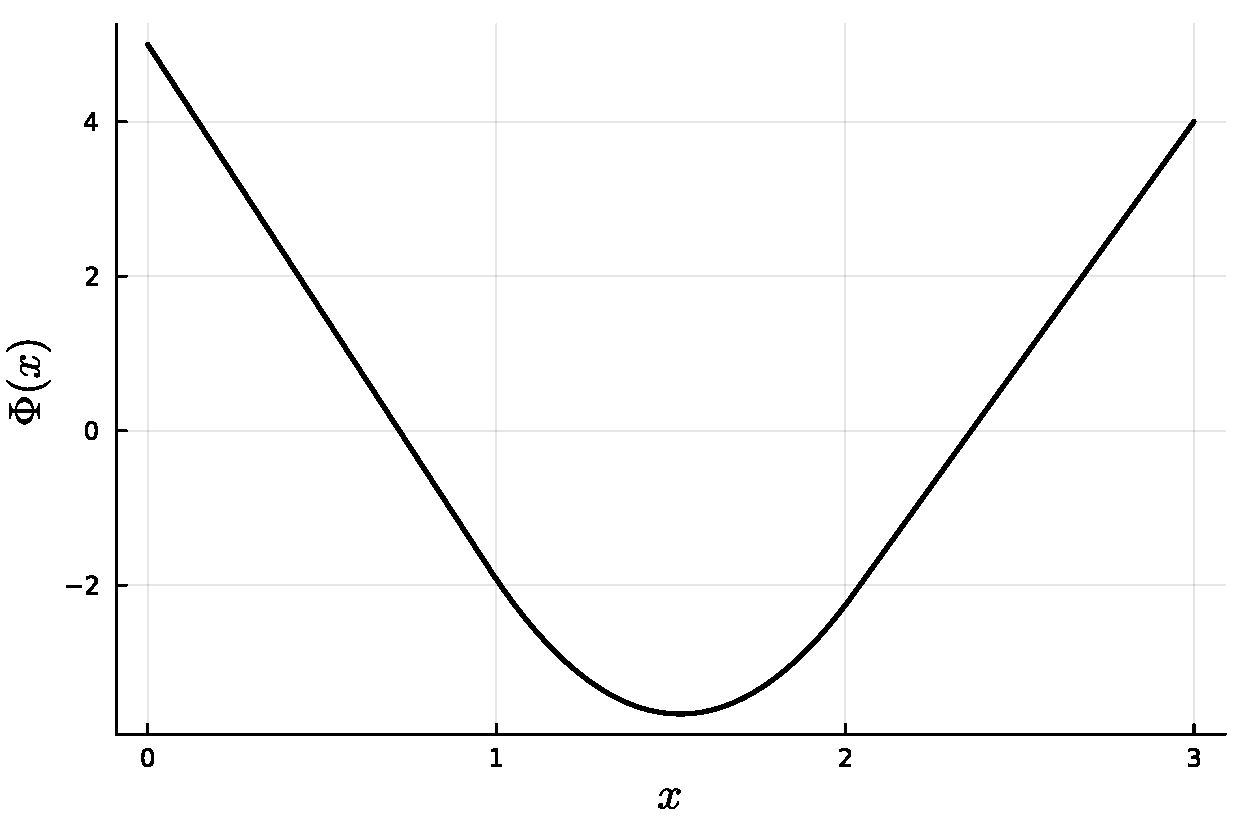
\includegraphics[width=0.8\textwidth]{../imgs/plot.pdf}
    \end{figure}
\end{document}